\chapter{3D Printed Components}

\section{Schematics of 3D Printed Mounts, Custom Components (Finalized Version)}

\newpage
    \begin{figure}[H]
        \centering
        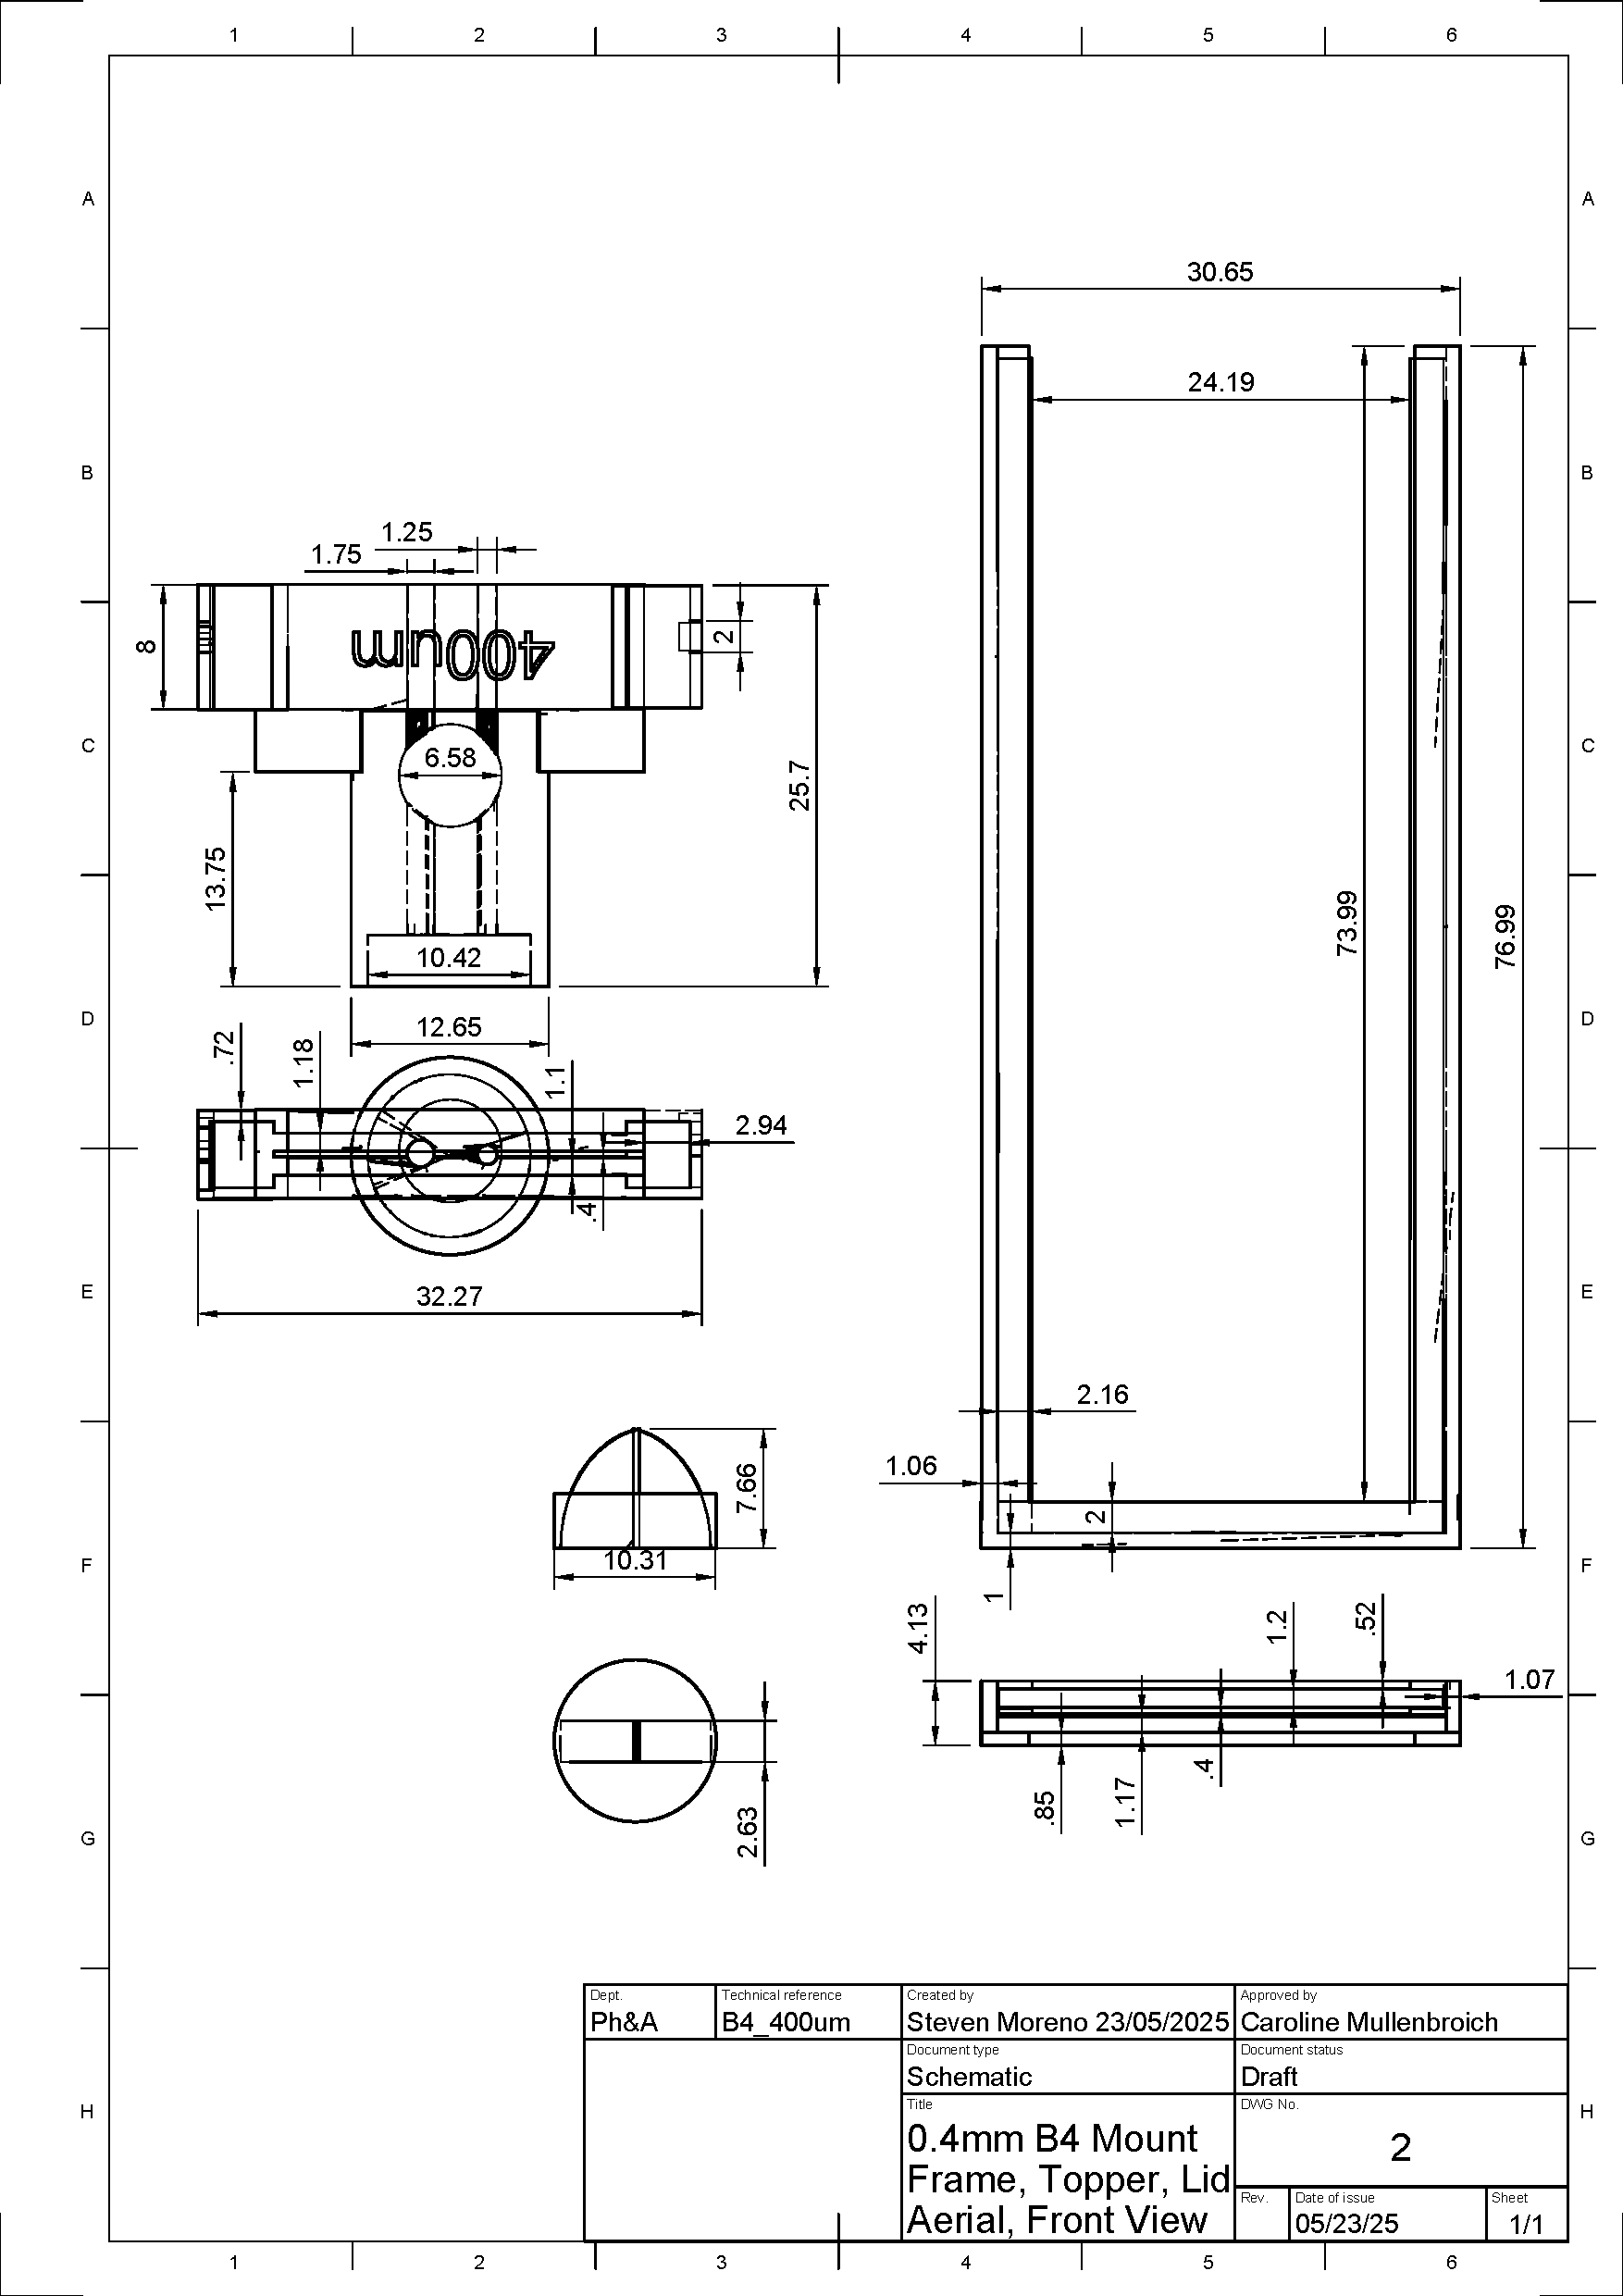
\includegraphics[width=1\linewidth]{Figures/0.4mm B4 Schematic v1.pdf}
        \caption{\textbf{Schematic of 3D Print B4 Mount for 0.4 mm Thick Tissue}}
        \label{fig:enter-label}
    \end{figure}
    
    \begin{figure}[H]
        \centering
        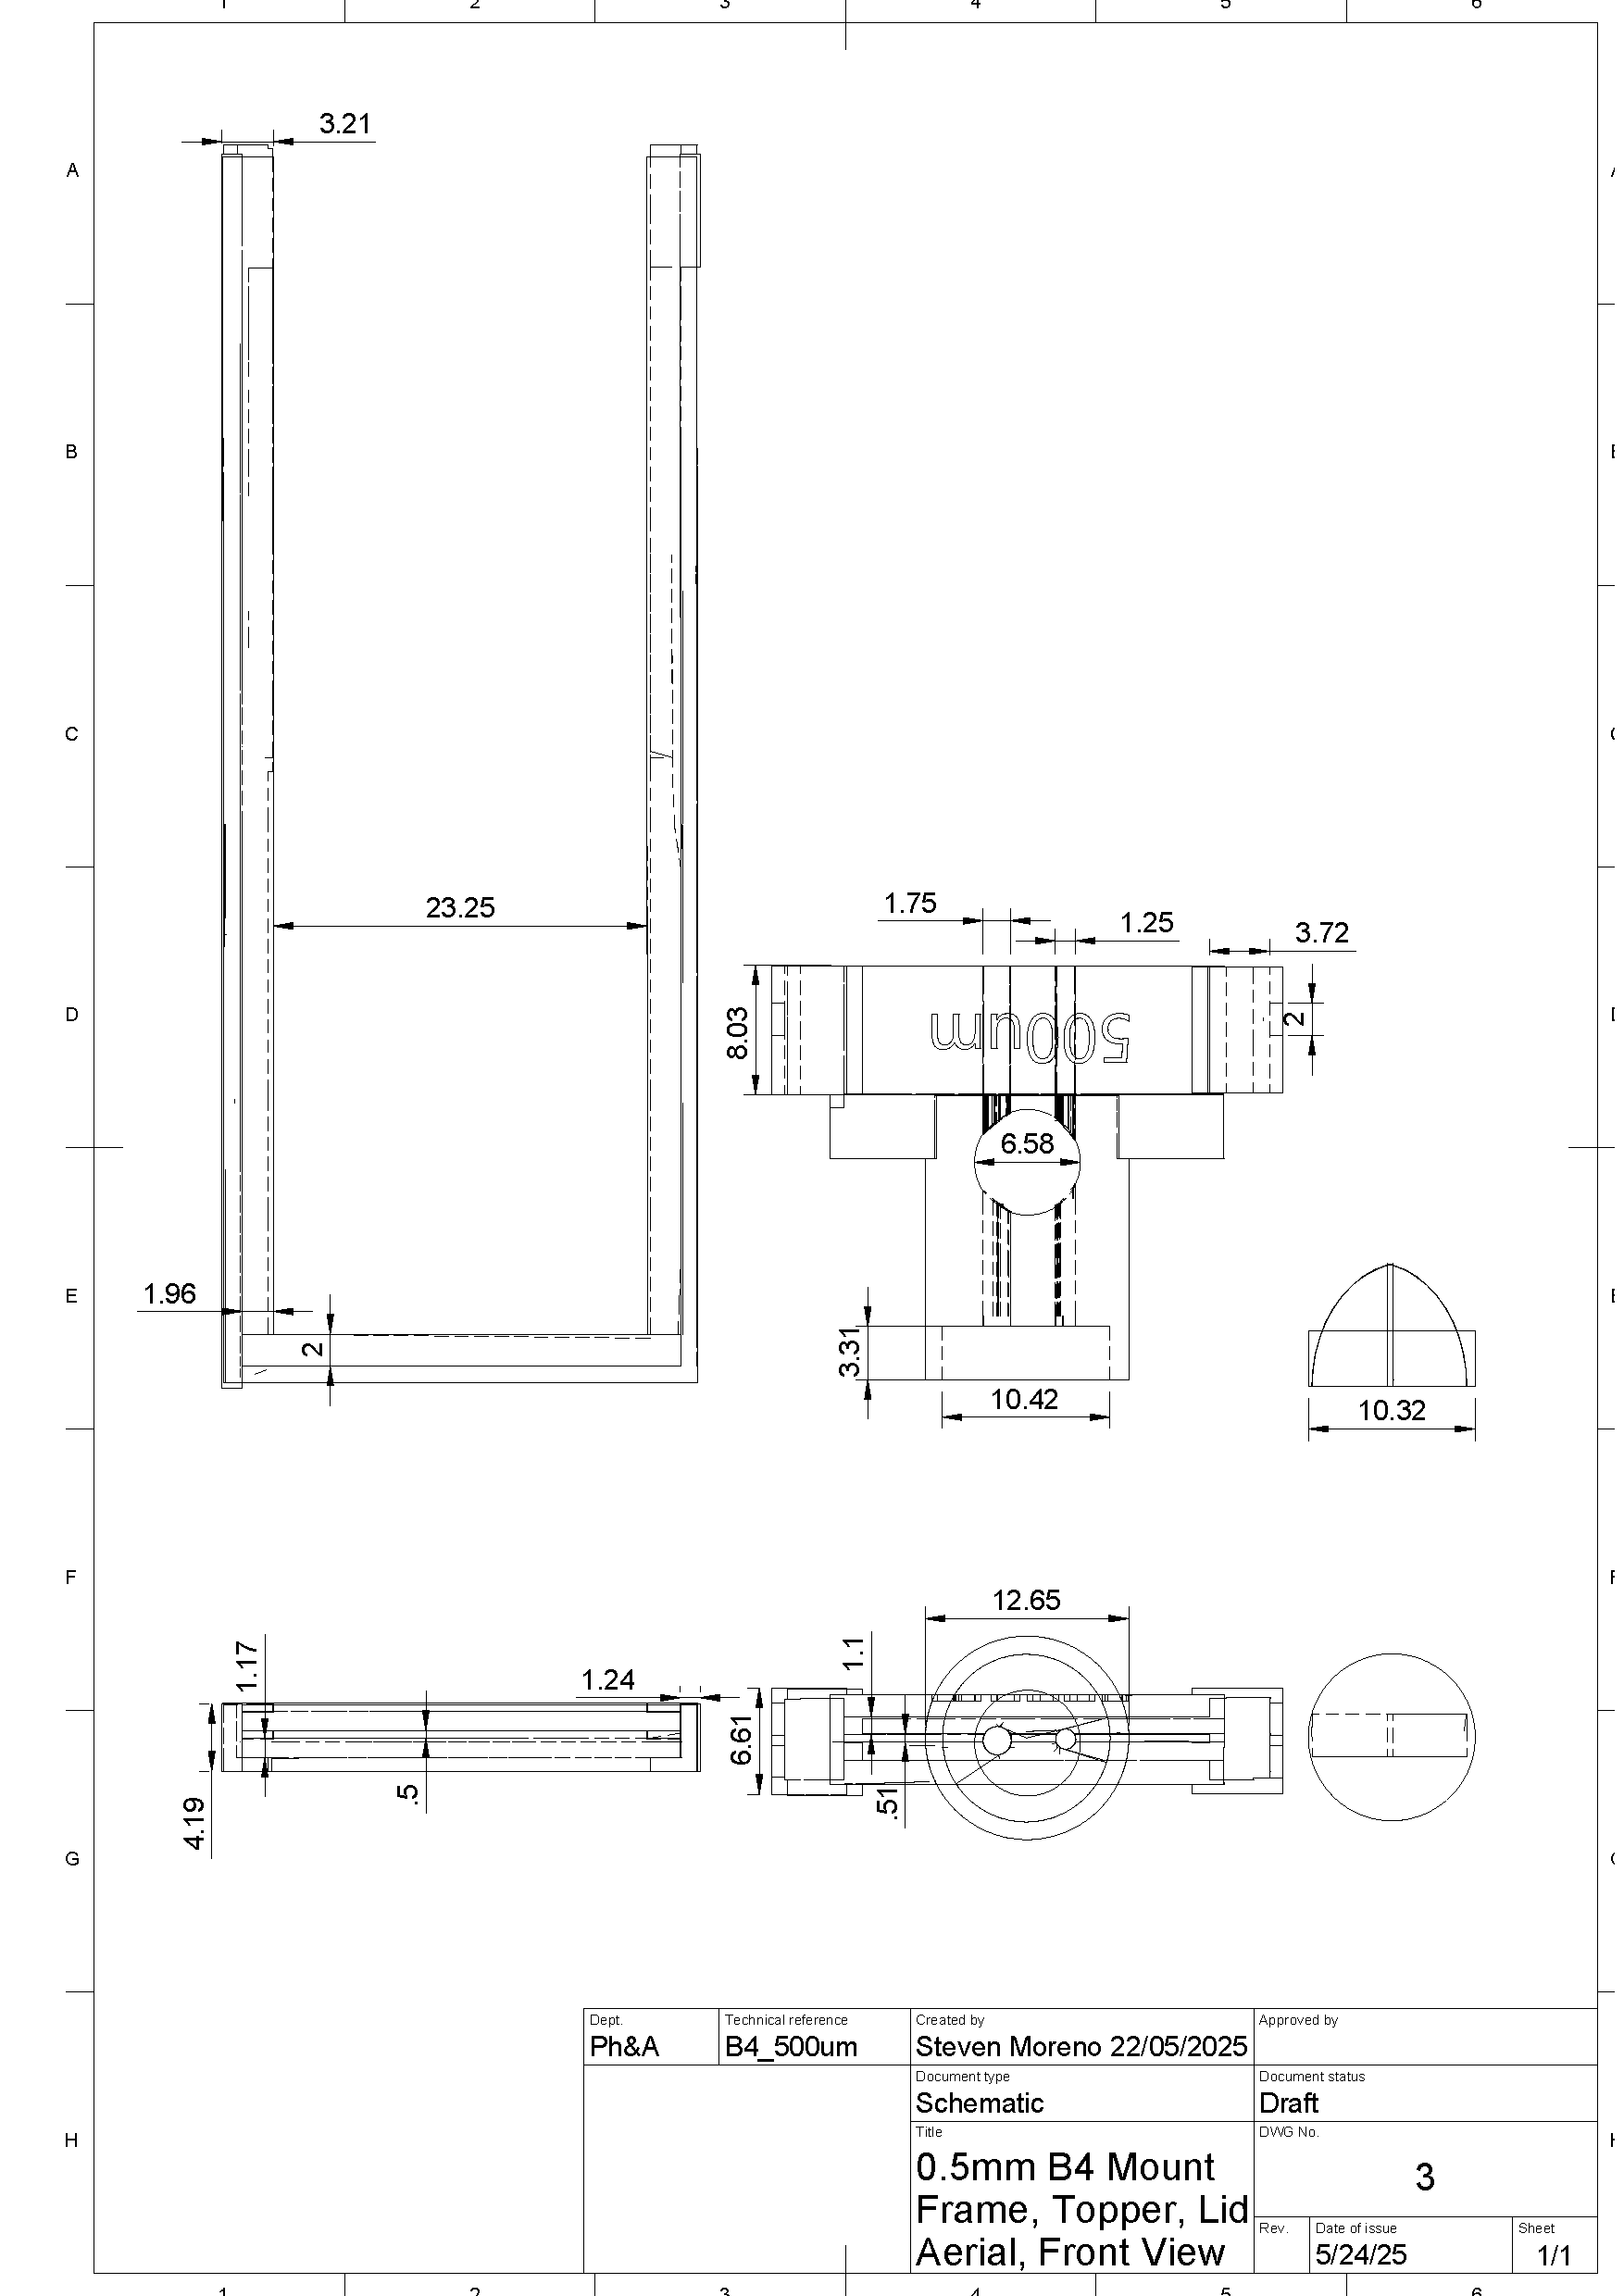
\includegraphics[width=1\linewidth]{Figures/0.5mmB4Schematic.pdf}
        \caption{\textbf{Schematic of 3D Print B4 Mount for 0.5 mm Thick Tissue}}
        \label{fig:enter-label}
    \end{figure}
    
    \begin{figure}[H]
        \centering
        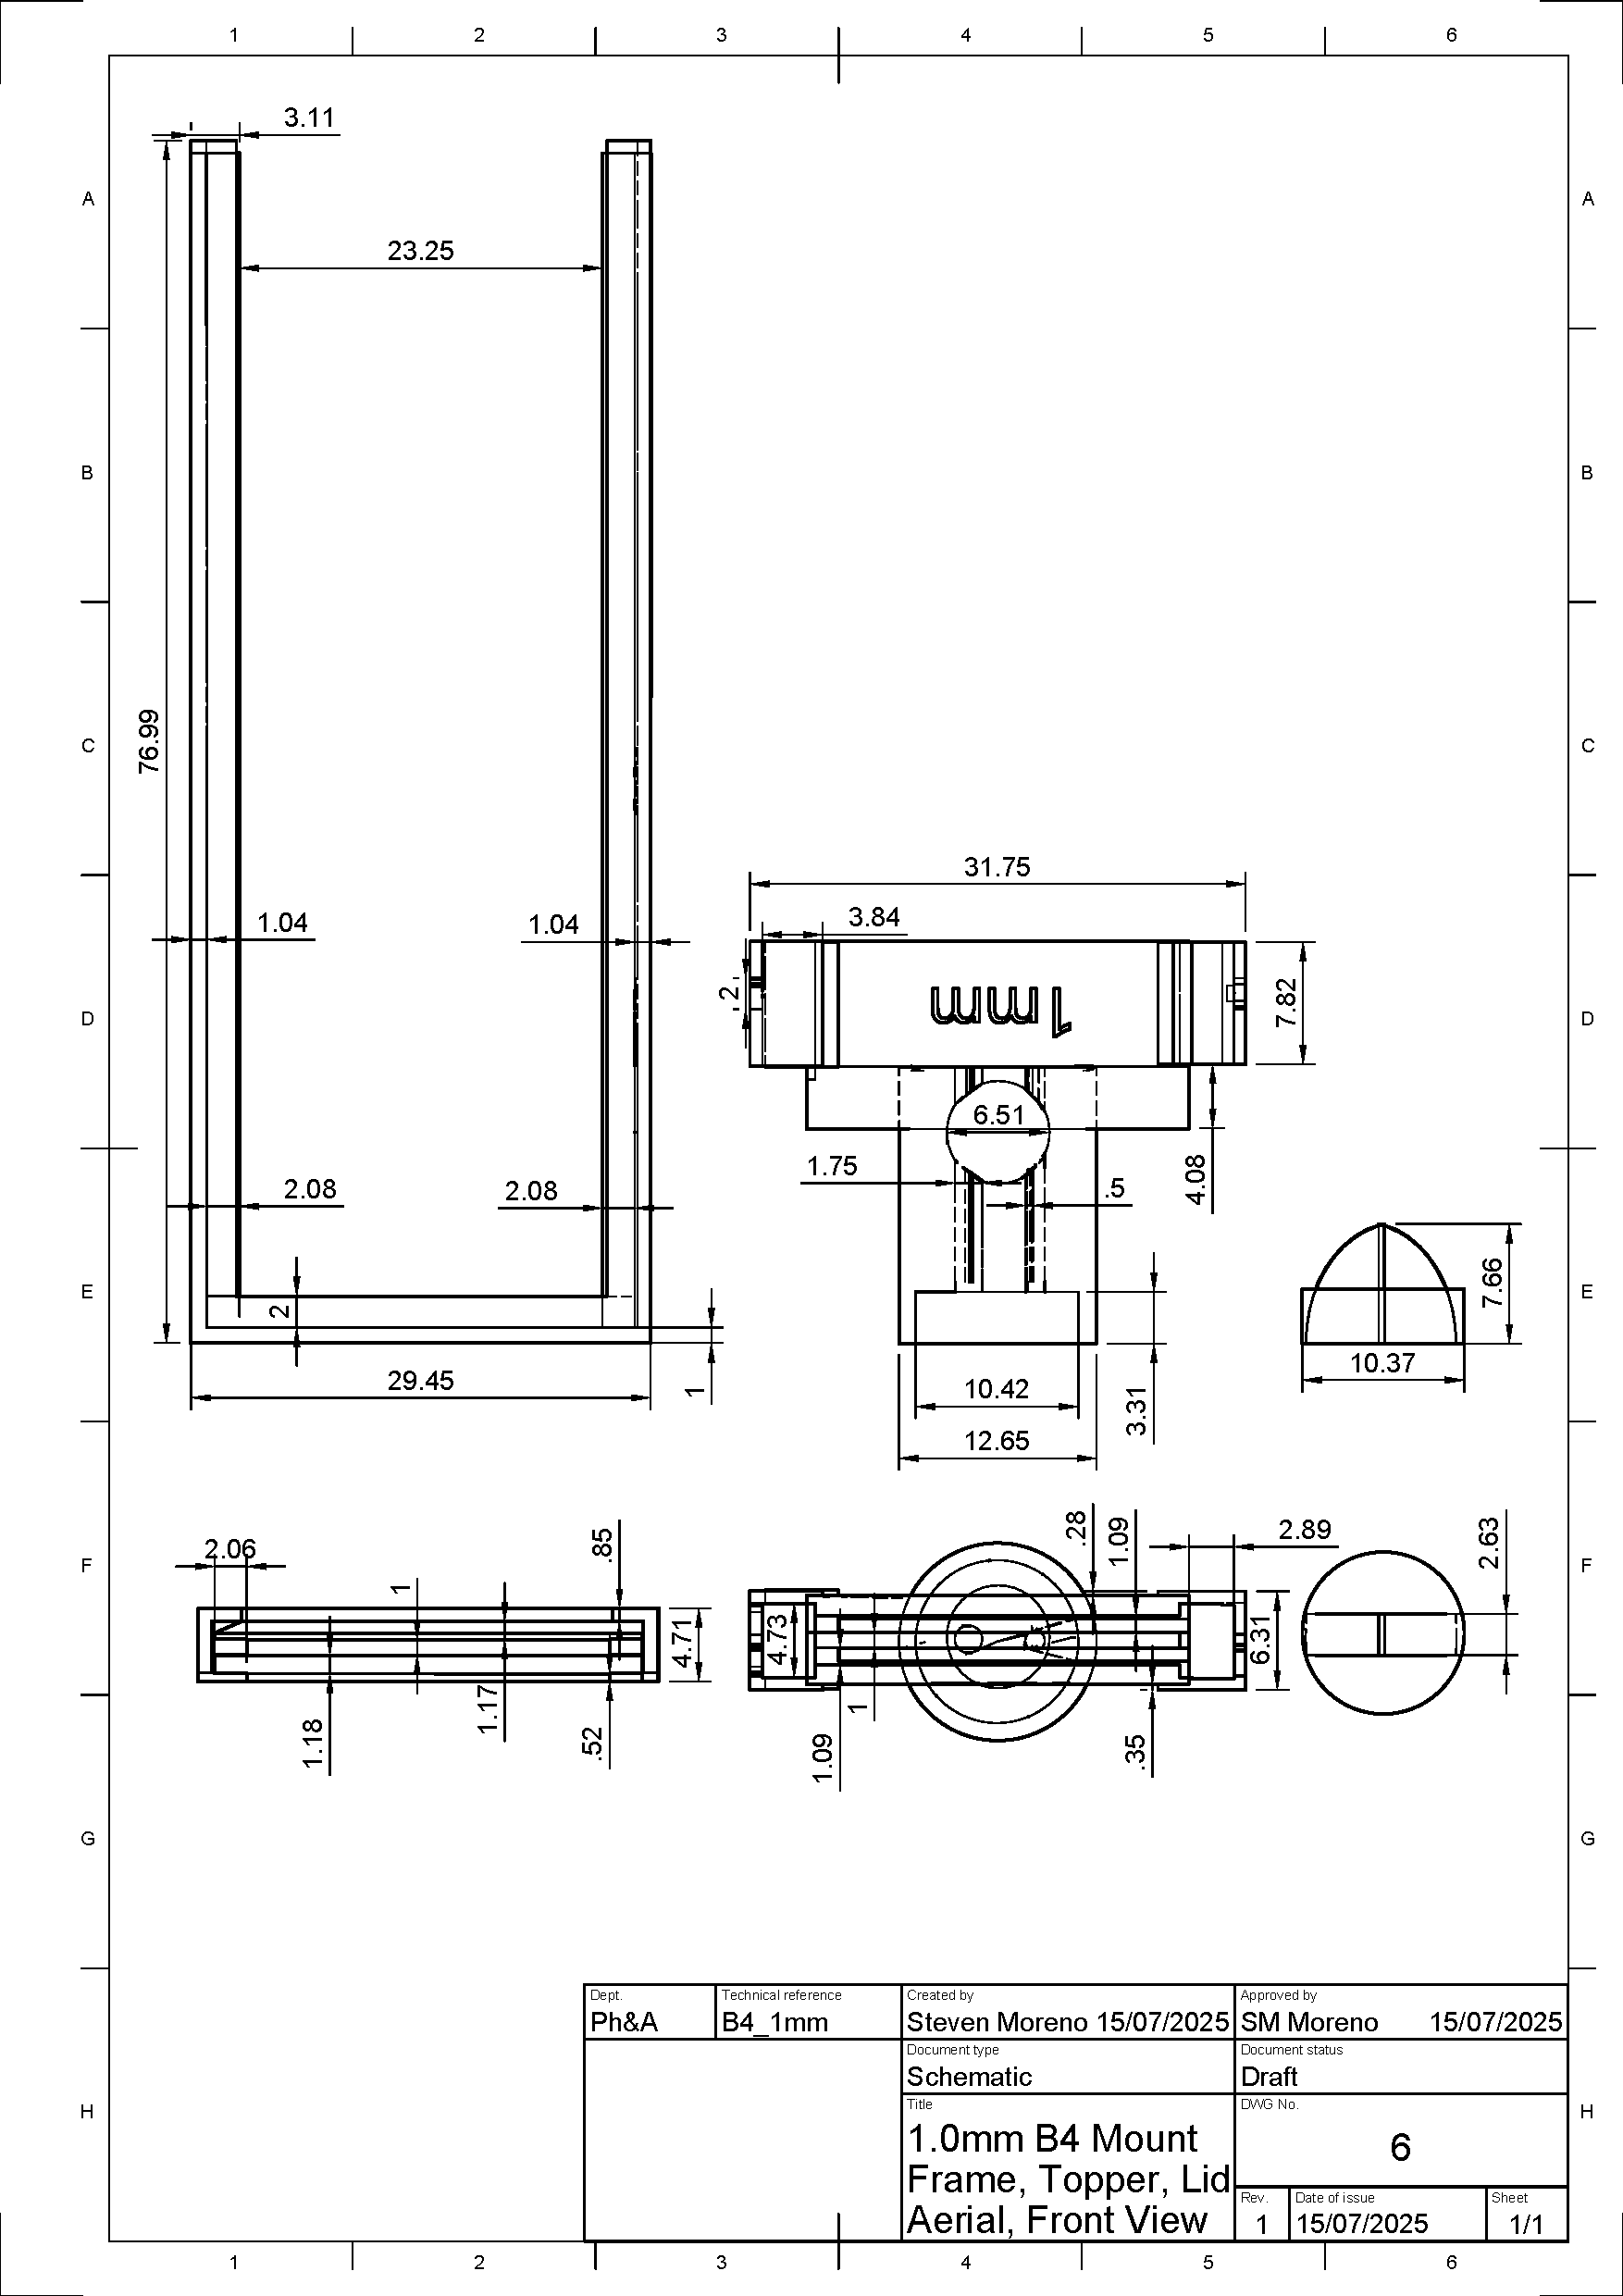
\includegraphics[width=1\linewidth]{Figures/1.0mm B5 Drawing v1.pdf}
        \caption{\textbf{Schematic of 3D Print B4 Mount for 1.0 mm Thick Tissue}}
        \label{fig:enter-label}
    \end{figure}
    
    \begin{figure}[H]
        \centering
        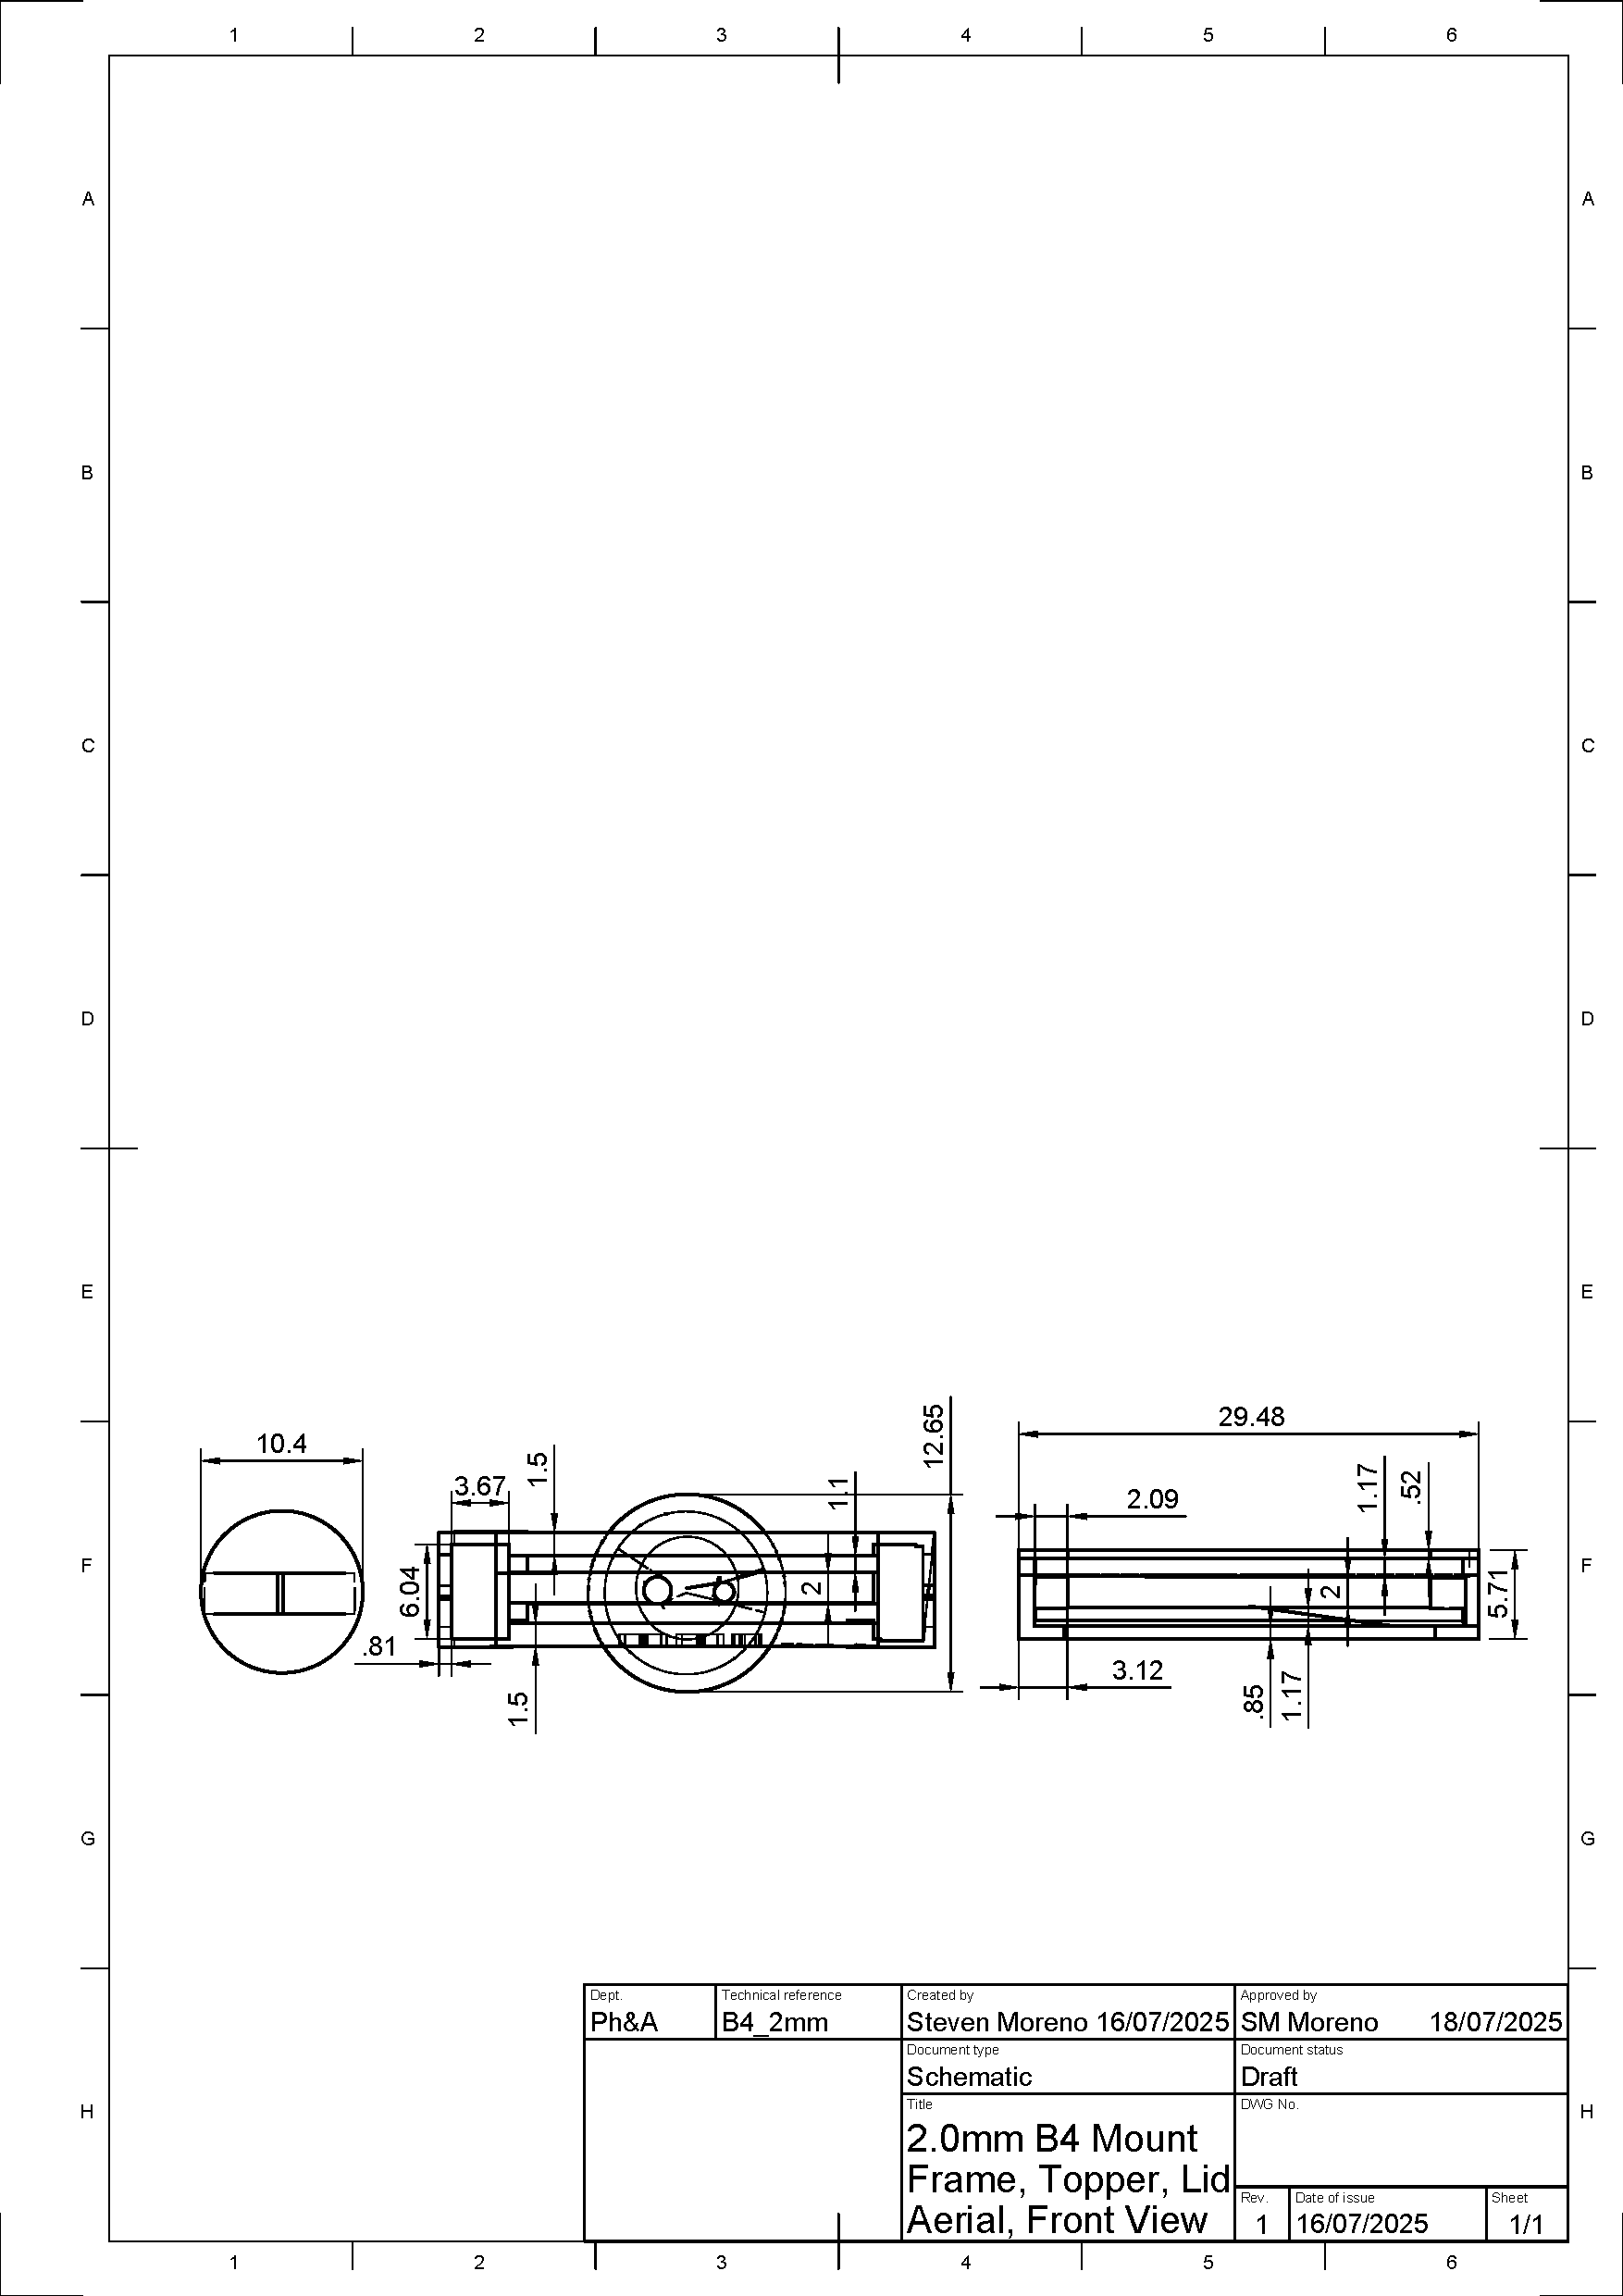
\includegraphics[width=1\linewidth]{Figures/2.0mm B5x2 Drawing v1.pdf}
        \caption{\textbf{Schematic of 3D Print B4 Mount for 2.0 mm Thick Tissue}}
        \label{fig:enter-label}
    \end{figure}
    
    \begin{figure}[H]
        \centering
        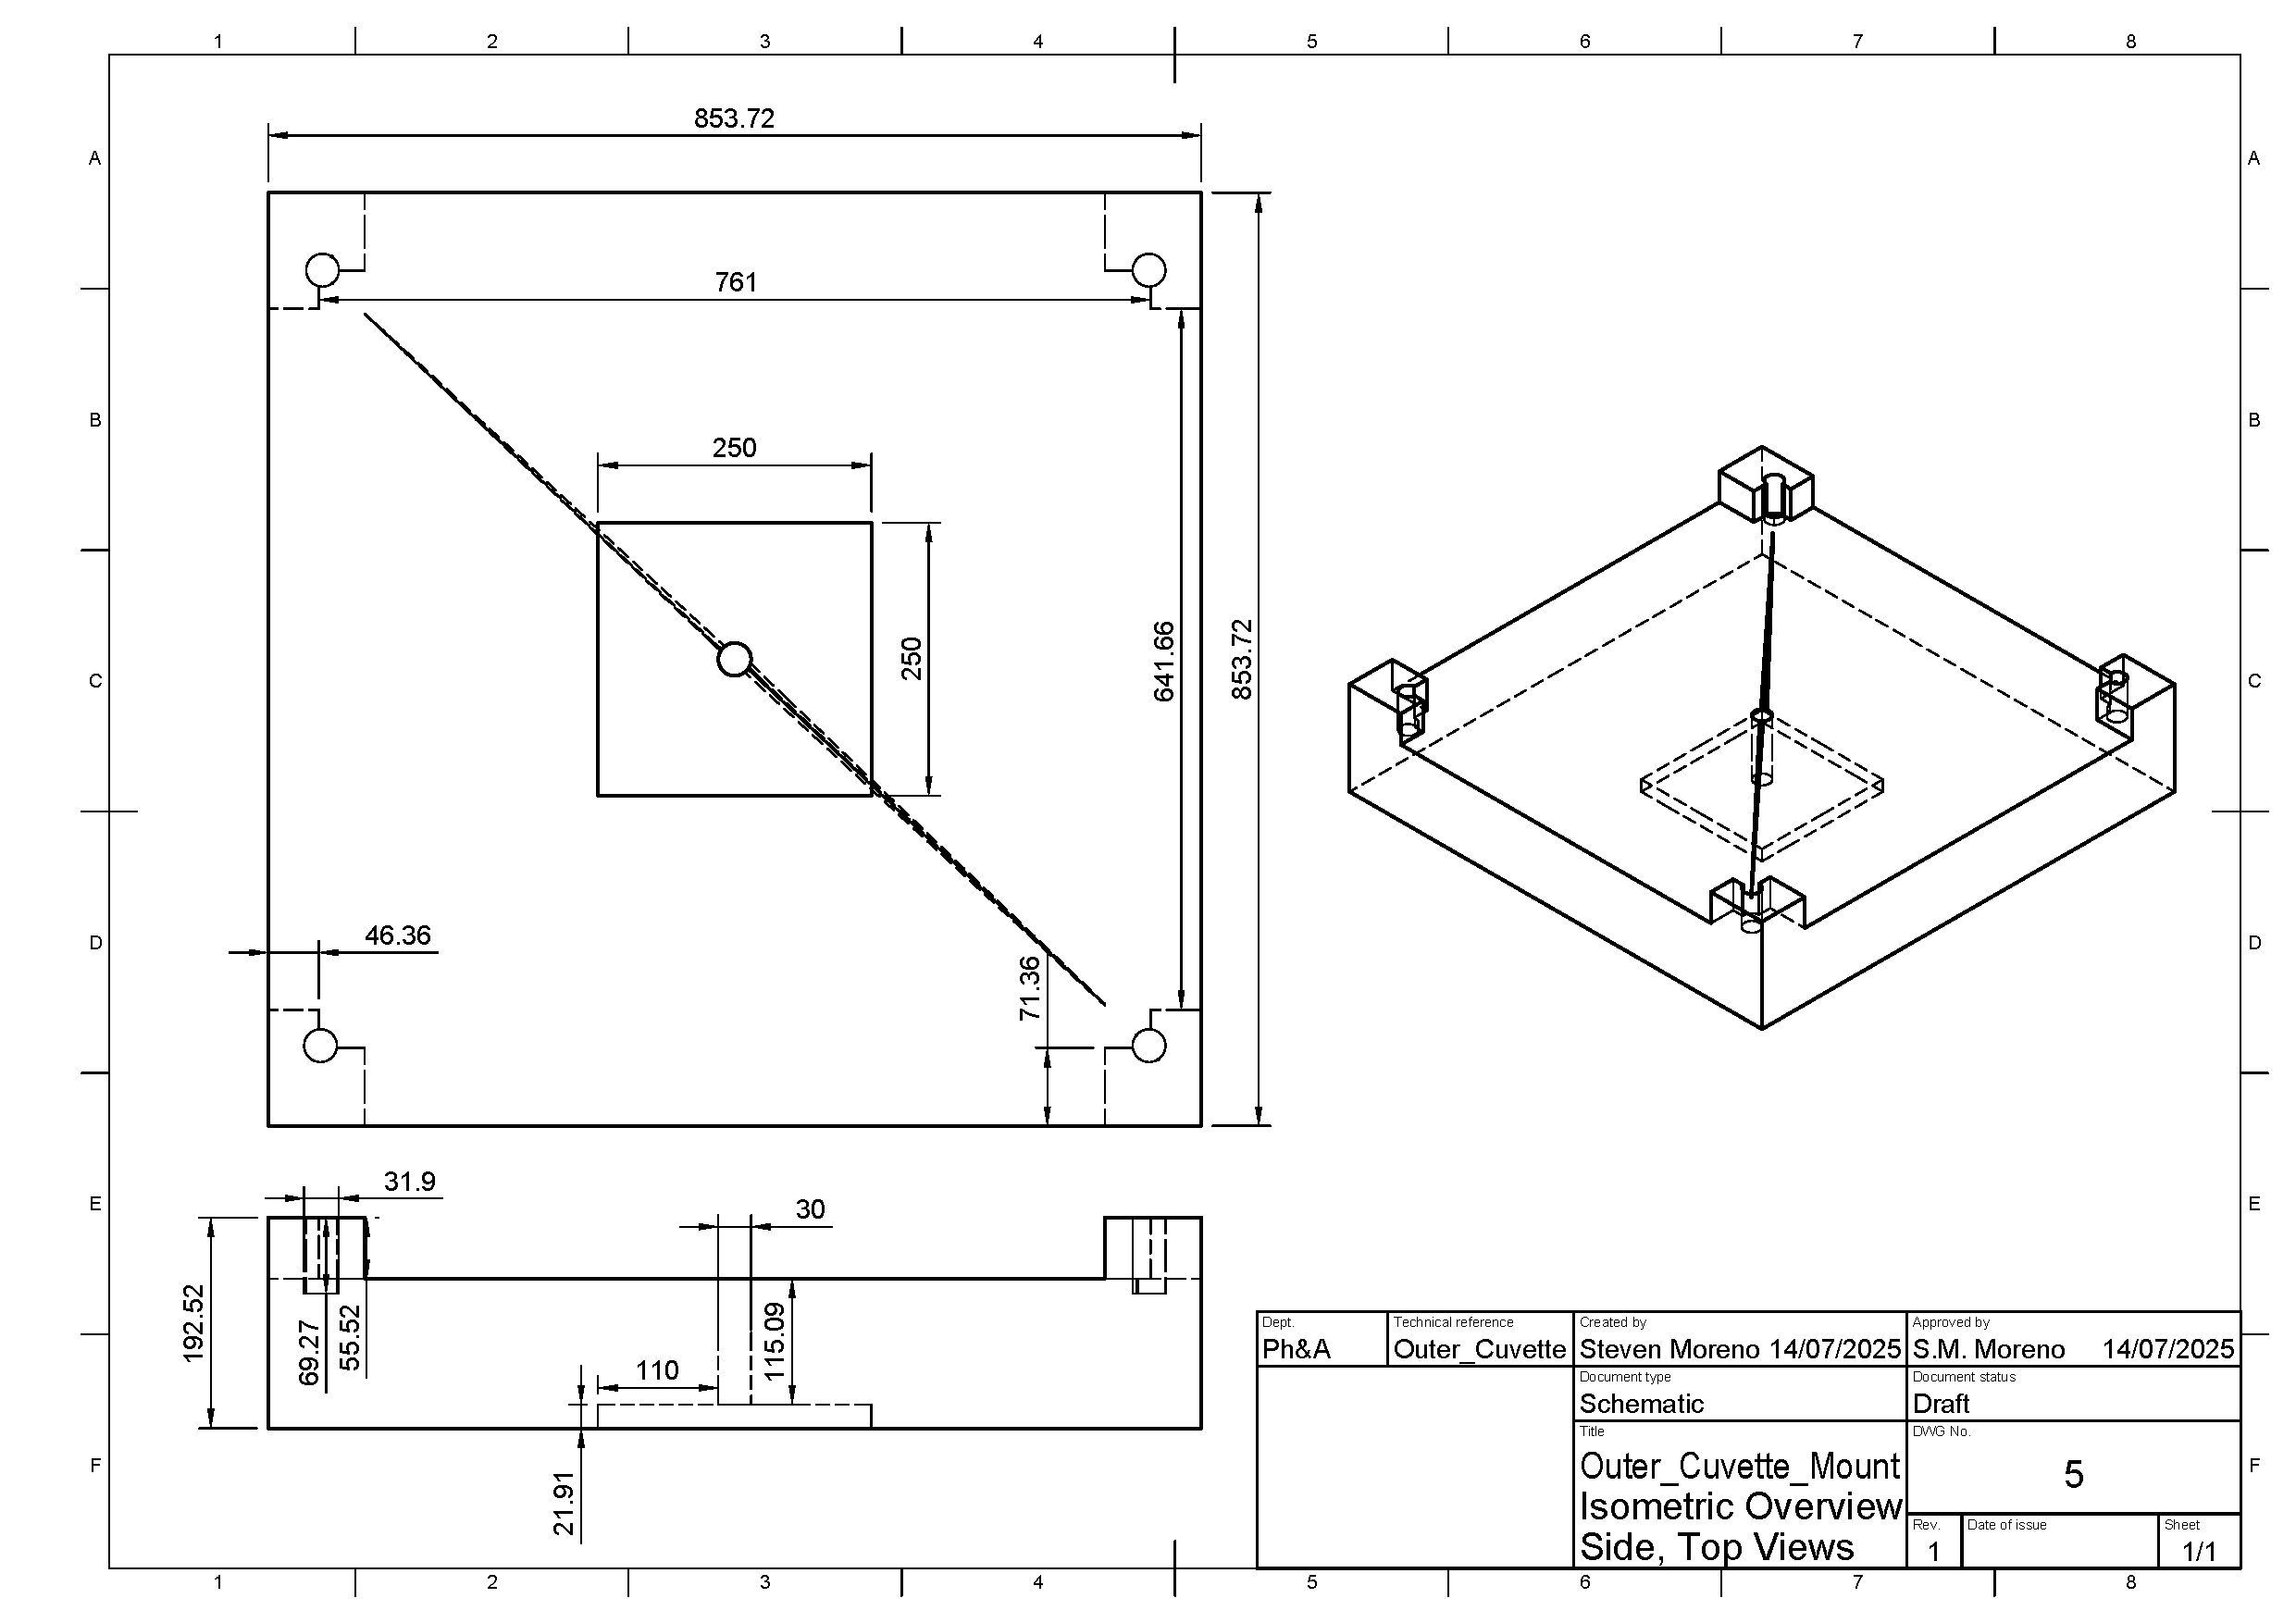
\includegraphics[width=1\linewidth]{Figures/Outer_Cuvette_Mount Drawing v1.pdf}
        \caption{\textbf{Schematic of 3D Print Custom External Cuvette Mount}}
        \label{fig:enter-label}
    \end{figure}
    
    \begin{figure}[H]
        \centering
        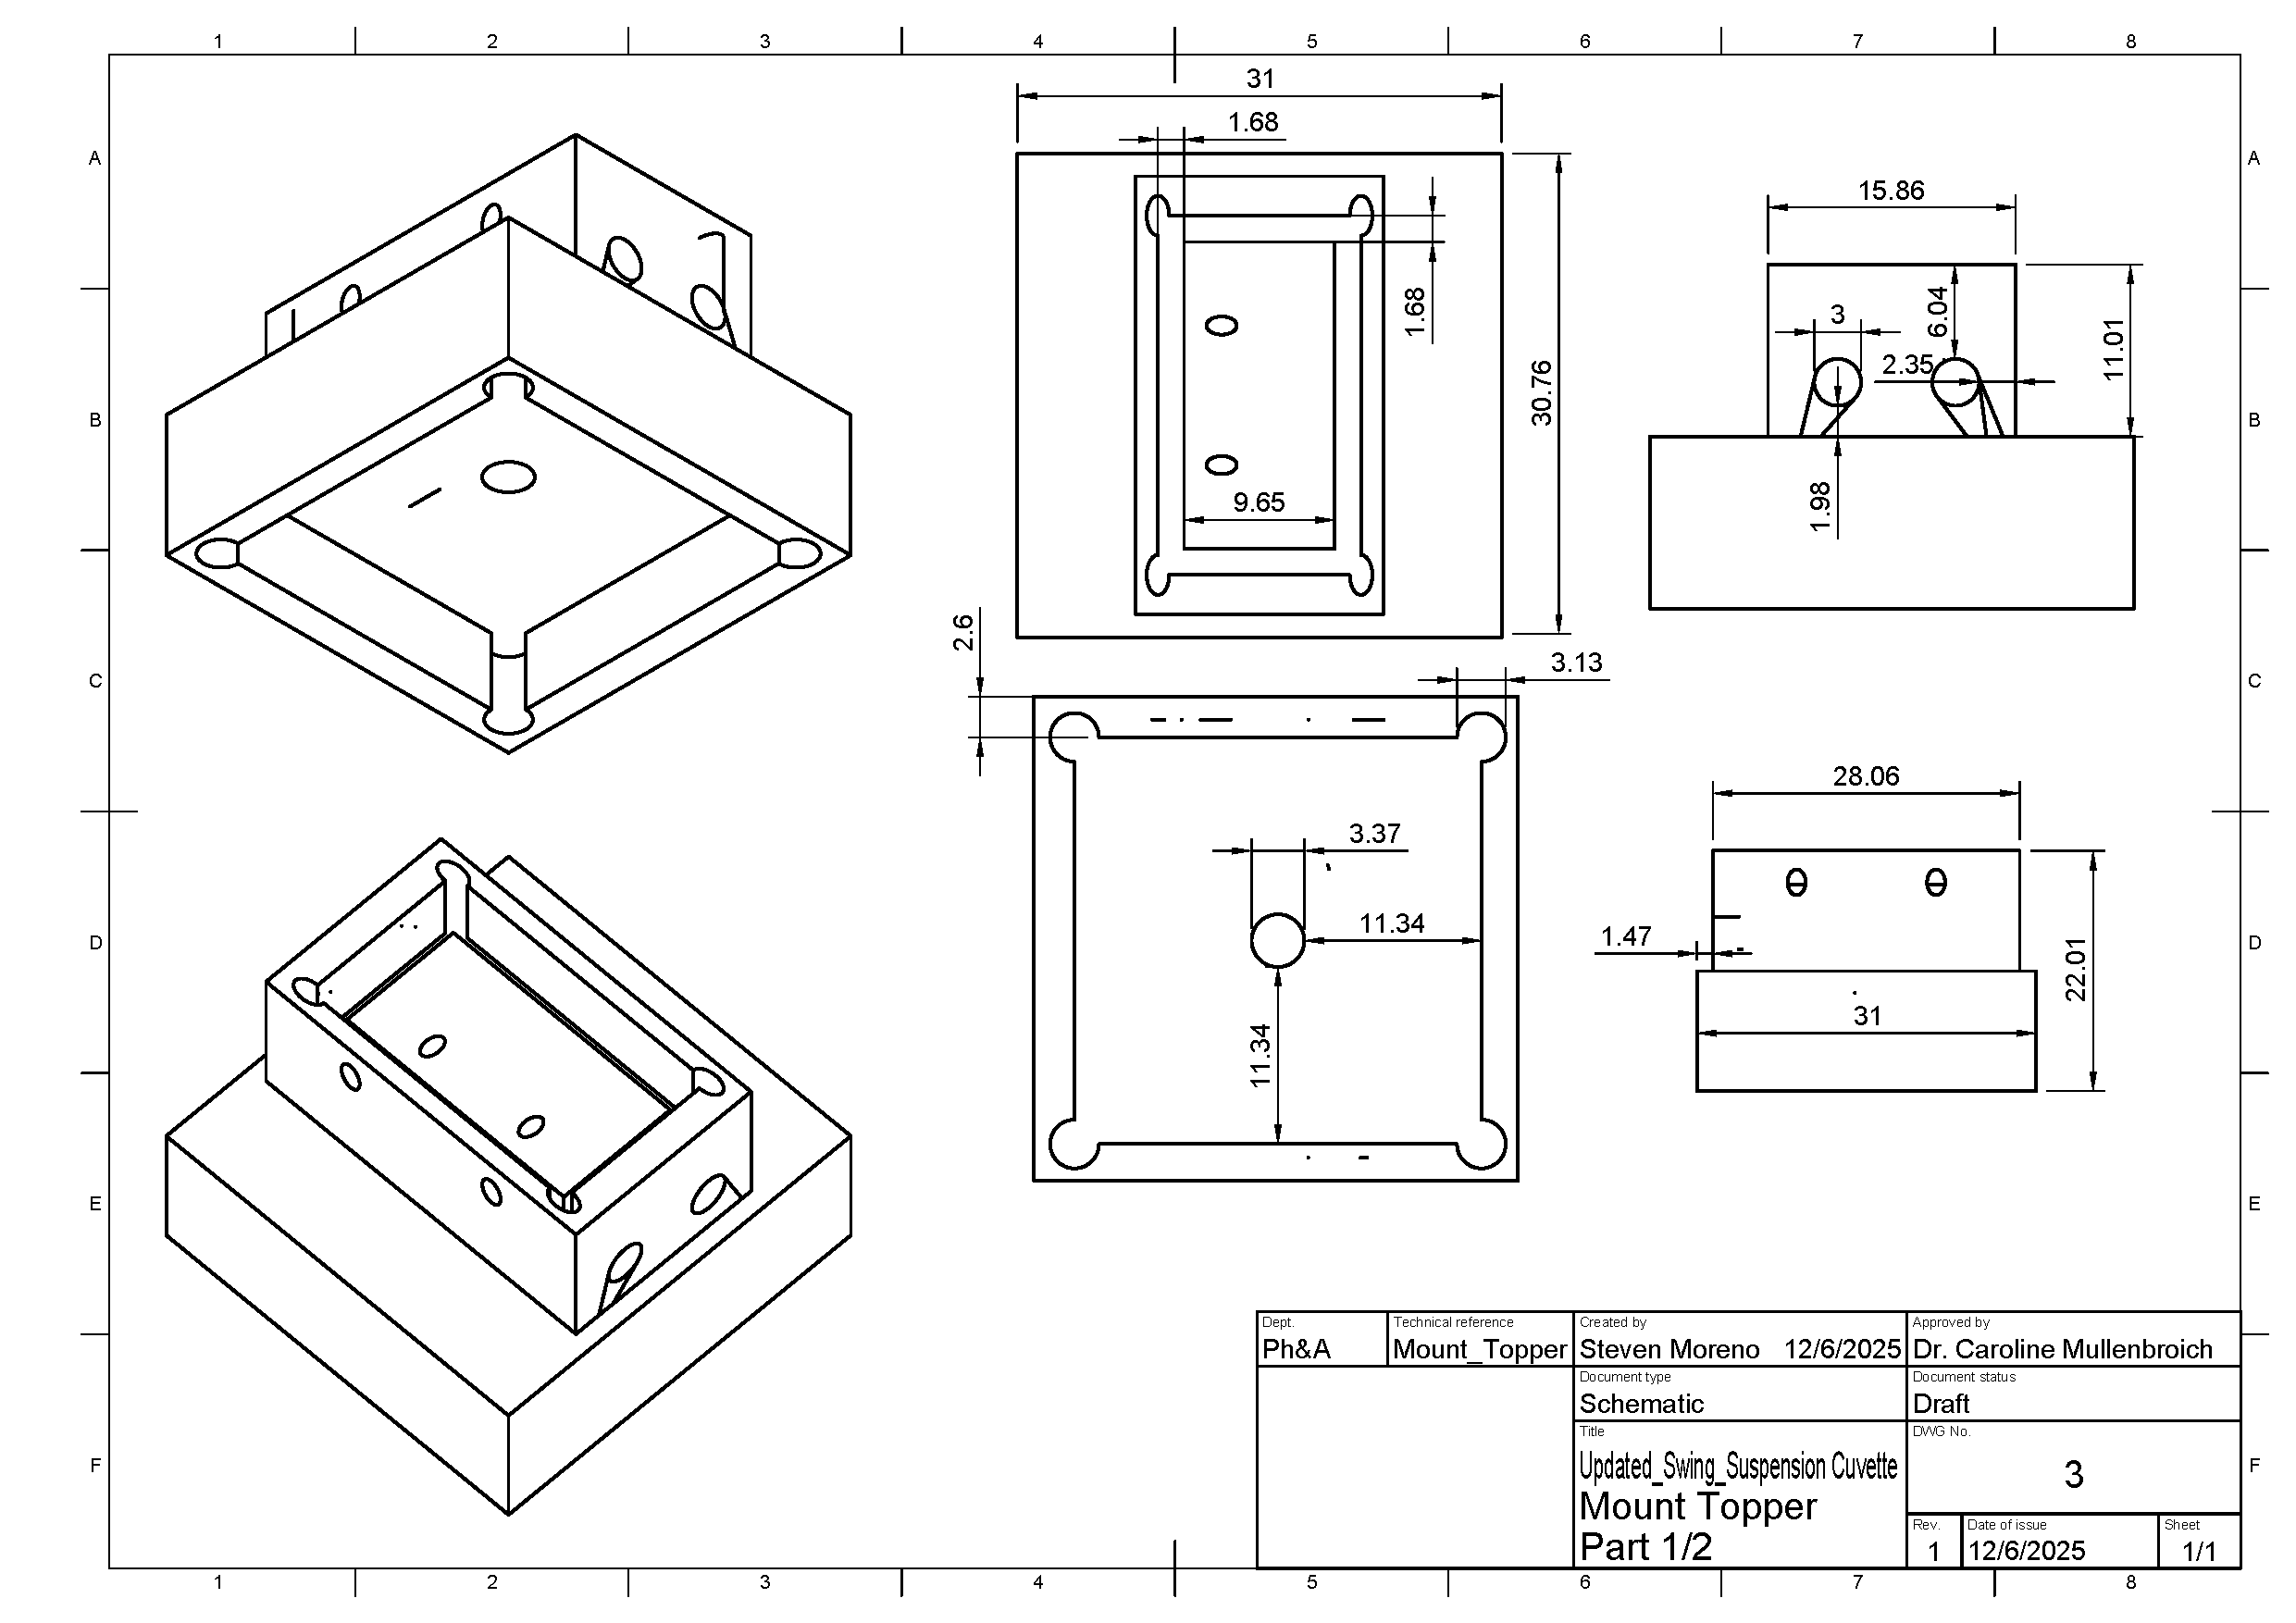
\includegraphics[width=1\linewidth]{Figures/Updated_Swing_Suspension Cuvette Topper Drawing v1.pdf}
        \caption{\textbf{Schematic of 3D Print Custom Internal Cuvette Mount Topper}}
        \label{fig:enter-label}
    \end{figure}

 \begin{figure}[H]
        \centering
        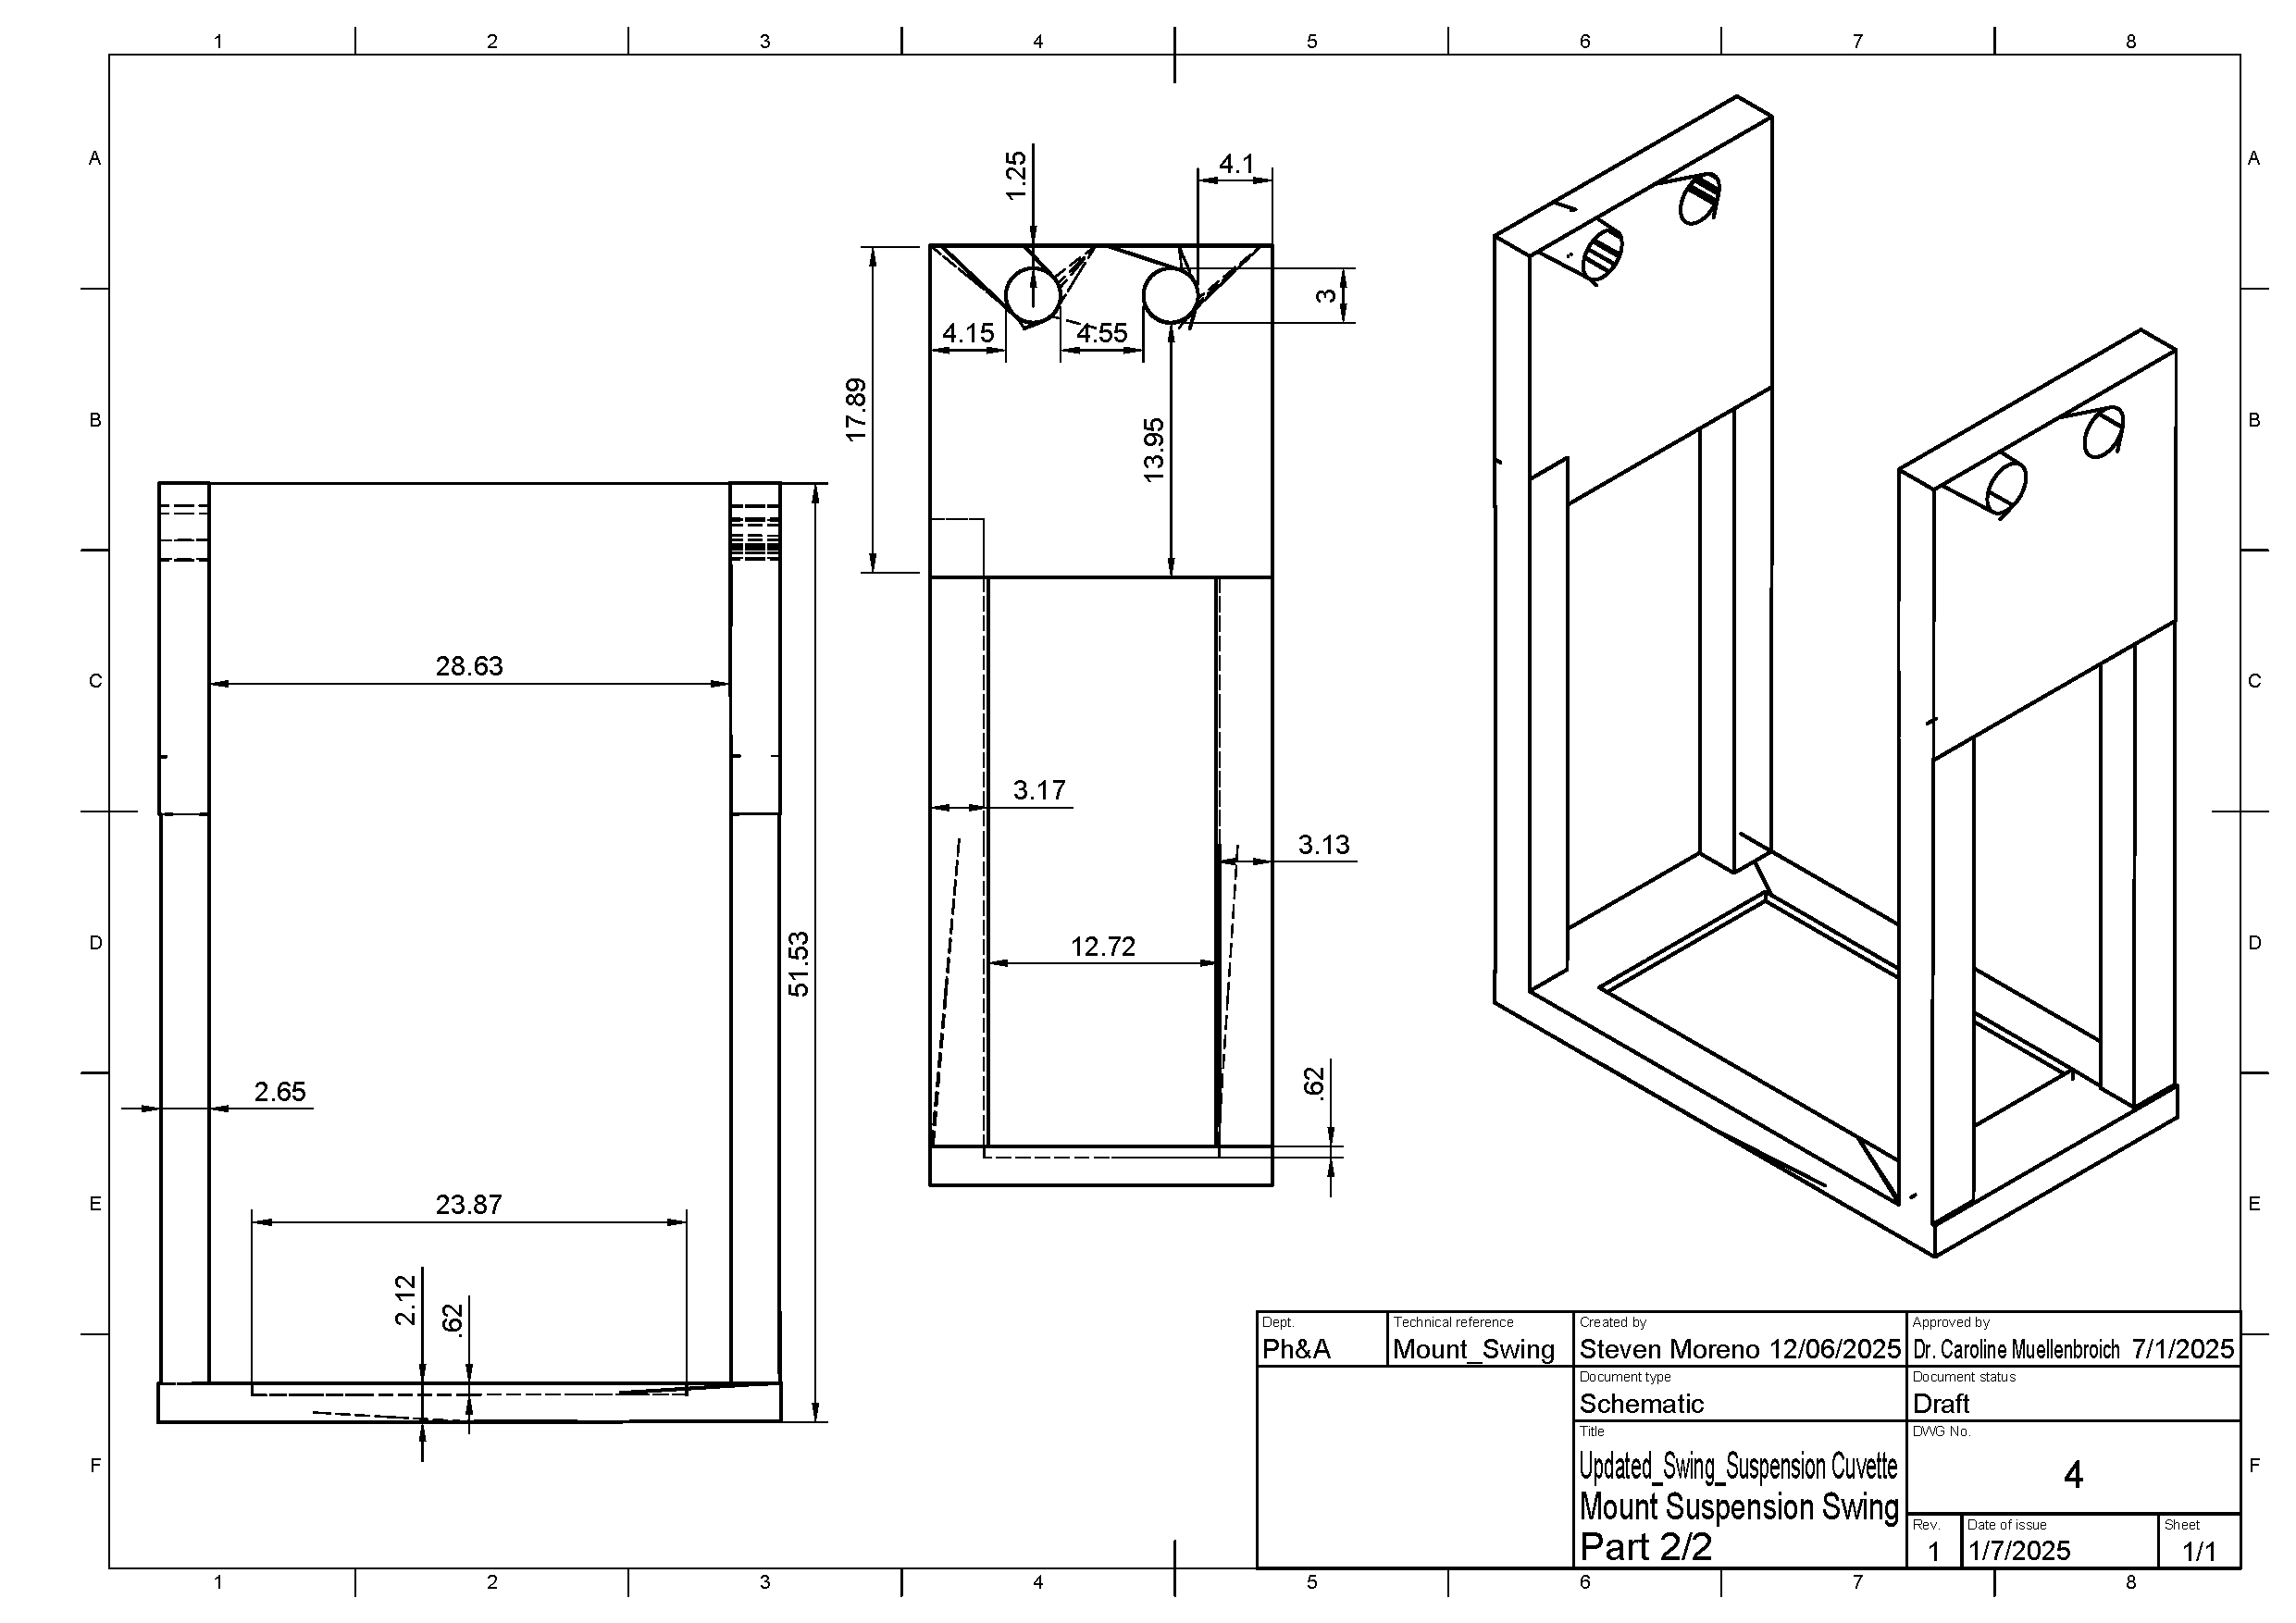
\includegraphics[width=1\linewidth]{Figures/Updated_Swing_Suspension Cuvette Swing v1.pdf}
        \caption{\textbf{Schematic of 3D Print Custom Internal Cuvette Mount Suspension Swing}}
        \label{fig:enter-label}
    \end{figure}
    
\vspace{0.5\textheight}

\section{3D Printer Settings and Code For 3D Printed Components}

3D printer files are available in a GitHub Repository created for files used in this project (URL HERE). For 3D printed components , files with printer settings preconfigured are available as .bgcode. Component files are also available as .stl files for adjustment of printer settings using 3D printer slicer programmes or adjustment of model dimensions using CAD software. Slicing and 3D printing was completed using Prusa Slicer ver 2.8.1 and MK4 Prusa Printer from Prusa Research, respectively.

\section{3D Models, Descriptions of 3D Printed Mount Iterations}
\subsection{First Generation of Tissue Mount Designs}

Initial Designs were based on spacers used in cardiac tissue clearing by Dr. Camilla Olianti [REF]. Dimensions were modified from her design to fit standard microscopy slide dimensions (76mm x 26mm x 1mm) and external ridges added to support slide placement while dual component silicone applied to the mount dries during mounting protocol. The mounts were printed as long, flat strands with 45 degree wedge shaped cuts added at 76mm and 102mm down the strand length to allow the mount to be folded manually into the desired 'U' shaped frame. This was done to ensure isotropic resolution of the mount spacer as the resolution of the 3D printer reduces considerably due to vibrations at higher z-axis planes with tall, narrow models. Basic suspension mounts toppers were designed which relied on friction between the coarse mount surface and the smooth mount glass surface to suspend the mount from above.


\begin{figure}[H]
        \centering
        
\includegraphics[width=1\linewidth]{Figures/Placeholder.png}
        \caption{\textbf{3D Models of First Generation of Tissue Mounting Spacers}}
        \label{fig:enter-label}
    \end{figure}
\subsection{Second Generation of Tissue Mount Designs}

After completing first session of tissue clearing and imaging with the first generation of mounts, multiple issues arose that required the mounts to be redesigned. First generation mounts were found to be too unstable, prone to breaking at the wedged cuts and often leaked from poor adhesion to the dual component silicone applied. Access to higher resolution 3D printers allowed for mounts to be printed vertically with no need to bend into position (See Appendix A.3 for details). An external sheathe was added to the internal mount to better hold the slides in place without risking damage to the sample inside. Injection ports were added to the mount toppers to allow for the injection of solutions and expulsion of air out of the mount without the need to remove the topper. 

\begin{figure}[H]
        \centering
        
\includegraphics[width=1\linewidth]{Figures/Placeholder.png}
        \caption{\textbf{3D Models of Second Generation of Tissue Mounts}}
        \label{fig:enter-label}
    \end{figure}
\subsection{Third Generation of Tissue Mount Designs}

Toppers designed in the first and second generation were prone to slipping, allowing mounts to partially slide off of the topper. Injection ports in these toppers were also prone to overflowing and bubble formation during injection of solution into the mounts. External sheathes were also found to be much more difficult to remove from the glass slides without breaking one or both in the process. Analysis of images recorded of mounts containing Agarose beads also confirmed the design of these mounts placed considerable strain on slides, which formed severe aberrations in images captured. These difficulties resulted in the third generation design which saw significant remodeling of the mount topper and internal mount. 

The mount topper was redesigned to wrap around the top 8mm of both the internal mount frame and slides to increase surface area available for static friction to occur. 2mm bore holes were added to the sides of the topper to allow for M2 bolts to be used for additional static friction support if needed. To reduce risk of overflows and bubbling experienced during injections, an 6.58mm diameter void was added inside the topper, between the injection and exhaust ports, to contain any splashes resulting from overflows or bubbling of solution. A lid was also created to cap off the entrance to the injection ports, which were now located inside a 3mm deep borehole on the top of the mount, to prevent entry of dust and other contaminates into the mount while in storage.   

The internal mount and external sheath were fused together into a single component and reduced in size to the narrowest dimensions it could be without losing the ability to form a watertight seal with dual component silicone. The upper half of the mount frame was closed off to reduce the impact vibrations would have on printing the upper half of the mount, maintaining the resolution of the model across all planes in the z-axis. 


\begin{figure}[H]
        \centering
        
\includegraphics[width=1\linewidth]{Figures/Placeholder.png}
        \caption{\textbf{3D Models of Third Generation of Tissue Mounts}}
        \label{fig:enter-label}
    \end{figure}

    
\subsection{Fourth/Final Generation of Tissue Mount Designs}
Further imaging attempts using Agarose bead samples confirmed the continued presence of aberrations in the images stemming from excess strain placed on the slides by the mount frame. It was determined through trial and error with a variety of prototype mount designs (each being a slight variation of the third generation design) that the cause of the strain was a combination of excessive dual component silicone applied to the mount and the closed off upper half of the mount frame applying pressure to the slides in opposite directions. 

The fourth and final design of the mount saw the removal of the closed off design of the upper half of the mount. In its place, scaffolding would be printed alongside the two tips of the mount frame to act as support frames mitigating the impact vibrations have on the resolution of the mount. In addition, the internal space inside the mounts where slides would be inserted into were increased in depth by approx. 0.2 mm to compensate for the reduction in resolution of the mount due to vibrations and to reduce strain placed on the slides by static friction experienced when inserted. No changes to design of the topper and lid were made.

Agarose bead tests with the fourth generation found aberrations caused by strain on the slides to be sufficiently mitigated. Further use of this design was found to work as intended with minimal issues, thus was selected to be the finalized mount design used in all experimental procedures for the remainder of the project. 

\begin{figure}[H]
        \centering
        
\includegraphics[width=1\linewidth]{Figures/Placeholder.png}
        \caption{\textbf{3D Models of Fourth/Final Generation of Tissue Mounts}}
        \label{fig:enter-label}
    \end{figure}